%!TEX root = main.tex

\begin{figure}[t]
  \centering
  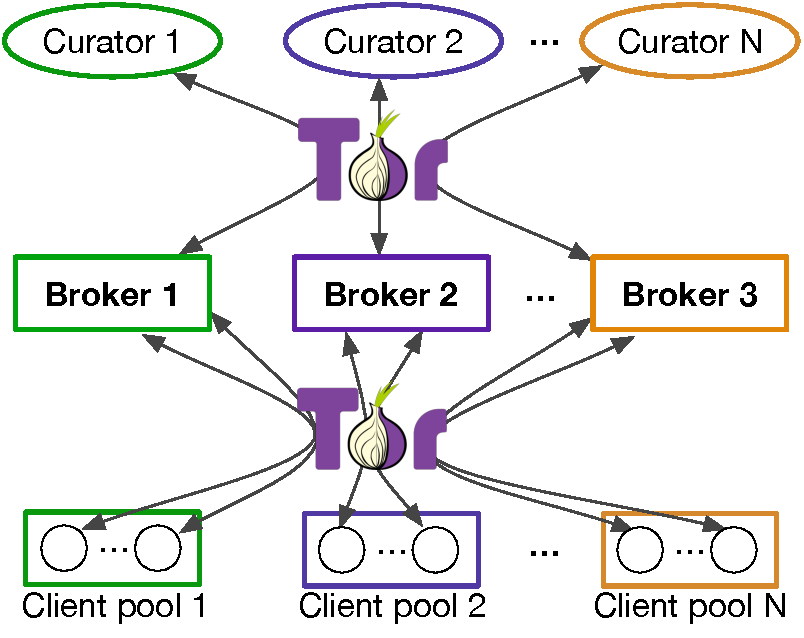
\includegraphics[width=.9\linewidth]{fig/sys-design-multib}
  \caption{Brokered learning and TorMentor design. Brokers
    (implemented as hidden Tor services) mediate between curators
    (top) and sets of clients (bottom). }
  \label{fig:sysdiagram}
\end{figure}


%%%%%%%%%%%%%%%%%%%%%%%%%%%%%%%%%%%%%%%%%%%%%%%%%%%%%%%%%%%%%%%%%%
\chapter{Brokered Learning}
\label{sec:setting}
%%%%%%%%%%%%%%%%%%%%%%%%%%%%%%%%%%%%%%%%%%%%%%%%%%%%%%%%%%%%%%%%%%

In this work, we define \textit{brokered learning}, which builds on the
federated learning setting~\cite{McMahan:2017}, but assumes no trust
between clients and curators.

\section{Decoupling federated learning}

In federated learning, a central organization (such as Google) acts as
the parameter server and performs two logically separate tasks:
\textbf{(1)} define the data schema and the learning objective, 
\textbf{(2)} coordinate distributed ML. The federated learning server
performs both tasks at a central service, however, there are good
reasons to separate them.

Fundamentally, the goals of data privacy and model accuracy are at
tension. Coordinating the ML training process in a private and secure
manner compromises the model's ability to learn as much as possible
from the training data. In current learning settings, the coordinator
is put in a position to provide privacy, yet they are not incentivized
to do so.

To take things even further, a malicious curator can observe the
contributions of any individual client, creating an opportunity to
perform information leakage~\cite{Hitaj:2017} attacks on clients, such
as model inversion~\cite{Fredrikson:2014, Fredrikson:2015} or
membership inference~\cite{Shokri:2017}. These attacks can be
mitigated in federated learning with a secure aggregation
protocol~\cite{Bonawitz:2017}, but this solution does not handle
poisoning attacks and requires several coordinated communication
rounds between clients for each iteration.

Client anonymity may also be desirable when privacy preferences are
shared. For example, if attempting to train a model that uses past
criminal activity as a feature, one user with strong privacy
preferences in a large group of users with weak privacy preferences
will appear suspicious, even if their data is not
revealed. 

% Furthermore, because curators in federated learning consume
% the final trained model, they are incentivized to optimize for
% accuracy in the accuracy-privacy trade-off.

A key observation in our work is that \emph{because data providers and model
curators agree on a learning objective before performing federated
learning, there is no need for the curator to also coordinate the
learning.}

\emph{Brokered learning} decouples the two tasks into two distinct
roles and includes mechanisms for anonymity to protect data providers
from the curator while orchestrating federated learning. In this
setting the users in the system (model curators and data providers) do
not communicate with one another, which facilitates a minimal trust
model, strengthening user-level privacy and anonymity. As well, users
do not reveal their personal privacy parameters to the broker, since 
\emph{all privacy-preserving computation is performed on the client}.

At the same time brokered learning maintains the existing privacy
features of federated learning: data providers do not need to
coordinate with each other (or even be aware of each other).
This is important to counter malicious clients who attack
other clients~\cite{Hitaj:2017}.

\section{Defining brokered learning}

\emph{Brokered learning} builds on federated 
learning~\cite{McMahan:2017} but provides additional privacy
guarantees. This model introduces a \textbf{broker} to mediate the
learning process. 

\textbf{Curators} define the machine learning model. A curator has a
learning task in mind, but lacks the sufficient volume or variety of
data to train a quality model. Curators would like to collaborate with
clients to perform the learning task and may want to remain
anonymous. We provide curators with anonymity in TorMentor by
deploying a broker as a Tor hidden service, and by using the broker
as a point of indirection (Figure~\ref{fig:sysdiagram}).

%% performing
%% privacy-preserving distributed machine learning over client datasets.

Curators may know the identities of clients that wish to contribute to
the model or may be unaware of the clients that match their learning
objectives. Brokered learning supports these and other use cases, For
example, curators may know some subset of the clients, or set a
restriction on the maximum number of anonymous clients who can
contribute\footnote{We assume that the broker identifies or advertises
the learning process to clients out of band, externally to TorMentor.}.

\textbf{Clients} contribute their data to the machine learning task
and specify the criteria for their participation. Instead of fully
trusting the curator as they would in federated learning, clients
communicate with an honest-but-curious broker. The broker is trusted
only with coordinating the learning process, and does not learn the
identity nor data of any client. This threat model is similar to what
was used in the secure aggregation protocol for federated 
learning~\cite{Bonawitz:2017}.

Brokered learning allows these clients to jointly contribute to a
shared global model, without being aware of nor trusting each other.
Each client only needs to be concerned about its personal privacy
parameters. Some clients may be more concerned with privacy than
others; brokered learning supports differentially private
machine learning with heterogeneous privacy levels, which has been
shown to be feasible~\cite{Geyer:2017}. 

% During training, the
% broker determines if each client's parameters are still being honored
% and takes the appropriate actions if they are not. This may involve
% pausing the stream of updates being passed to a model from a specific
% client, or pausing the entire learning process and waiting for some
% conditions to be met before proceeding. 

\textbf{A broker} is a short-lived process that coordinates the
training of a multi-party ML model. When a model that is defined by a
curator in TorMentor, a single broker is created and deployed as a
hidden service in an anonymous network \footnote{In this paper we do not
  consider who is running the broker; but we do assume that it is
  an honest-but-curious third party that is distinct from the
  curator and the participating clients.}.
%
Clients perform actions such as requesting access to the system, defining
client-specific privacy parameters and sending model updates for
distributed SGD. We define a precise client \ac{API} in 
Section~\ref{sec:design}. When model training is complete, the broker
publishes the model and terminates. In our vision, brokers are not
intended to be long lasting, and their sole function should be to
broker the agreement between users to facilitate anonymous multi-party
ML. Brokers may even explicity be managed by governments or as part of
a privacy enhancing business model, both of whom are incentivized to
provide privacy, anonymity and fairness in distributed ML.

% Then, we detail TorMentor's design and
% implementation in Sections~\ref{sec:design} and~\ref{sec:impl}. We
% evaluate our prototype in Section~\ref{sec:eval}.

\section{Example use cases}

\noindent \textbf{Medical Sharing Network}. Hospitals store substantial
patient medical data. However, due to strict regulations, they 
cannot share this data with each other. No individual
hospital wishes to host the infrastructure for model coordination, and
no individual hospital is trusted to securely coordinate the analysis.
An alternative solution is for the network of hospitals to collaborate in
a brokered learning system. For this the hospitals would define the
learning task, one hospital would agree to deploy the broker as a
hidden service, and all other willing hospitals would join and
contribute model updates, training a shared model. \\

\noindent \textbf{Internet of Things}. With the growth of the Internet
of Things (IoT), and a largely heterogeneous set of device providers,
there is currently no solution for privacy-preserving multi-device ML,
hosted by a neutral provider. Without anonymous multi-party ML, each
system device provider would need to host their own ML coordinators and
would have no mechanism for sharing models across other providers. 

Brokered learning allows these devices to collaborate on model training
without explicitly trusting each other. Devices reap the benefits of
shared trained models, without risking data privacy loss. The broker
can be run by any single company, or a neutral trusted third party,
neither of which have power to compromise device-level privacy.

